\documentclass[../TDO4.tex]{subfiles}%

\begin{document}
\section[s]"2"{Étude d'un photocopieur}
\enonce{%
	Un photocopieur permet la formation de l'image d'un document sur une surface
	photosensible par l'intermédiaire d'un objectif de reproduction. On désire
	reproduire un document de format A4 soit en A4 (même format), soit en A3
	(format double en surface) soit en A5 (format moitié en surface).
	\bigbreak
	On réalise ces différents tirages à l'aide d'un objectif en modifiant la
	position respective des lentilles à l'intérieur du système. La distance
	entre le document et le récepteur photosensible est de \SI{384}{mm} et l'on
	positionne une première lentille mince divergente $\Lc_1$ de distance focale
	image $f'_1 = \SI{-90}{mm}$ à \SI{180}{mm} du récepteur
	(Figure~\ref{fig:phot-a}).
	\smallbreak
	\noindent
	\begin{minipage}{0.48\linewidth}
		\begin{center}
			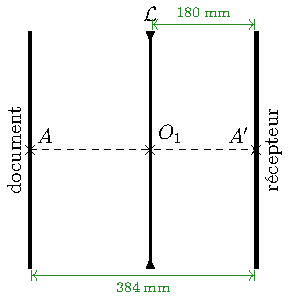
\includegraphics[width=.9\linewidth]{photocopieur-a}
			\captionof{figure}{Situation 1.}
			\label{fig:phot-a}
		\end{center}
	\end{minipage}
	\begin{minipage}{0.48\linewidth}
		\begin{center}
			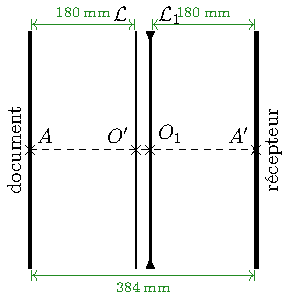
\includegraphics[width=.9\linewidth]{photocopieur-b}
			\captionof{figure}{Situation 2.}
			\label{fig:phot-b}
		\end{center}
	\end{minipage}

}%

\QR{%
	La lentille $\Lc_1$ peut-elle donner une image du document sur le
	récepteur ?
}{%
	La lentille divergente ne peut pas donner une image réelle si l'objet
	est réel (vérifiez avec la relation de conjugaison). Par conséquent,
	l'image à travers $\Lc_1$ \textbf{ne peut pas être sur le récepteur},
	car cette dernière est virtuelle.
}%

\QR{%
	On ajoute une lentille mince $\Lc'$ devant la lentille $\Lc_1$, à
	\SI{180}{mm} du document
	(Figure~\ref{fig:phot-b}). La lentille
	$\Lc'$ peut-elle être divergente ? Justifier votre réponse.
}{%
	Si $\Lc'$ est divergente, l'image de A est virtuelle, comme vu précédemment~;
	mais ça sera donc un objet réel pour $\Lc_1$, et on a encore le même
	raisonnement. Ainsi, si une lentille peut fonctionner dans ce système, elle ne
	peut être divergente.
}%

\QR{%
	Calculer la distance focale image $f'$ de cette lentille $\Lc'$
	pour obtenir une image réelle du document sur le récepteur. Pour
	cela, on utilisera deux relations de Descartes.
}{%
	L'image finale est telle que $\obarr{O_1A'} = \SI{180}{mm}$, l'objet
	initial est tel que $\obarr{O'A} = \SI{-180}{mm}$ et on a
	$\obarr{O'O_1} = \SI{24}{mm}$. Avec le système $\rm A
		\opto{\Lc'}{\rm O'} A_1 \opto{\Lc_1}{\rm O_1} A'$, on sait qu'on a les
	relations
	\begin{equation*}
		\left\{
		\begin{aligned}
			\frac{1}{f'}   & = \frac{1}{\obarr{O'A_1}} -
			\frac{1}{\obarr{O'A}}
			\\
			\frac{1}{f'_1} & = \frac{1}{\obarr{O_1A'}} -
			\frac{1}{\obarr{O_1A_1}}
		\end{aligned}
		\right.
		\Lra
		\left\{
		\begin{aligned}
			f'             & = \left( \frac{1}{\obarr{O'A_1}} -
			\frac{1}{\obarr{O'A}} \right)^{-1}
			\\
			\obarr{O_1A_1} & = \left( \frac{1}{\obarr{O_1A'}} -
			\frac{1}{f'_1} \right)^{-1}
		\end{aligned}
		\right.
		\Lra
		\left\{
		\begin{aligned}
			f'             & =
			\frac{\obarr{O'A_1}\times\obarr{O'A}}
			{\obarr{O'A}-\obarr{O'A_1}}
			\\
			\obarr{O_1A_1} & = \frac{f'_1\times\obarr{O_1A'}}
			{f'_1-\obarr{O_1A'}}
		\end{aligned}
		\right.
	\end{equation*}
	On en déduit
	$\DS\obarr{O'A_1} =
		\obarr{O_1A_1} - \obarr{O_1O'} =
		\frac{f'_1\times\obarr{O_1A'}}
		{f'_1-\obarr{O_1A'}} - \obarr{O_1O'}$~; avec
	$ \left\{
		\begin{array}{rcl}
			f'_1          & = & \SI{-90}{mm} \\
			\obarr{O_1A'} & = & \SI{180}{mm} \\
			\obarr{O_1O'} & = & \SI{-24}{mm}
		\end{array}
		\right.$ on a
	\[
		\xul{\obarr{O'A_1} = \SI{84}{mm}}
	\]
	et finalement avec $\obarr{O'A} = \SI{-180}{mm}$, on a également
	\[
		\xul{f' = \SI{57}{mm}}
	\]
}%

\QR{%
	En déduire le grandissement $\gamma$ de l'association des deux
	lentilles et indiquer quel type de tirage permettra cet objectif~:
	transformer du A4 en A3 ou du A4 en A5 ?
}{%
	$\gamma\ind{imprim} = \gamma_{\Lc'}\gamma_{\Lc_1}$ en tant
	qu'association de lentilles~; or $\gamma_{\Lc'} =
		\dfrac{\obarr{O'A_1}}{\obarr{O'A}} = \num{-0.5}$,
	et $\gamma_{\Lc_1} =
		\dfrac{\obarr{O_1A'}}{\obarr{O_1A_1}} = 3$~: on a
	\[
		\xul{\gamma\ind{imprim} = \num{-1.5}}
	\]
	$|\gamma\ind{imprim}| > 1$ d'une part, mais pour savoir si on peut
	imprimer en A3 il faut savoir si la \textit{surface} est multipliée par
	2~; $\gamma$ est un grandissement linéique (sur une longueur). Pour la
	surface, on calcule $\gamma\ind{imprim}^2 = 2.25 > 2$~: on peut donc
	transformer du A4 en A3.
}%

\end{document}
